
\providecommand{\myrootdir}{..}
\documentclass[\myrootdir/main.tex]{subfiles}

\begin{document}

\chapter{Our Information Extraction Tool}
\label{implementation}
describe implemantation of Tool
\includegraphics[page=7, width=\textwidth, trim={0.5cm 0.5cm 0.5cm 0.5cm}, clip]{img/flow-of-research.pdf}

\section{Common Interface} 
unification tool, reference CLI somehow nicely?,

ruby tool, unifies different syntax command line interfaces of the other tools, easy to switch between different techniques (NOT TOO LONG)

\section{PROSE Program Synthesis}
implementation details :)

C\#, based on PROSE Text Extraction DSL, parsing example set files, feeding learning session \& applying learned regex program, can do single string extraction and also sequence extraction \& showing differentiating examples (although not in use)

\section{IR Similarity}
impl details,

R, text2vec, tokenized vectors, impl of preprocessing?

don't repeat from IE models section!

\section{Keyword search}
impl details,

R, simple!

\end{document}
